\section{Komponenten}

\subsection{Physische Komponenten}

\subsubsection{Intel RealSense D435}

\begin{figure}[hbt!]
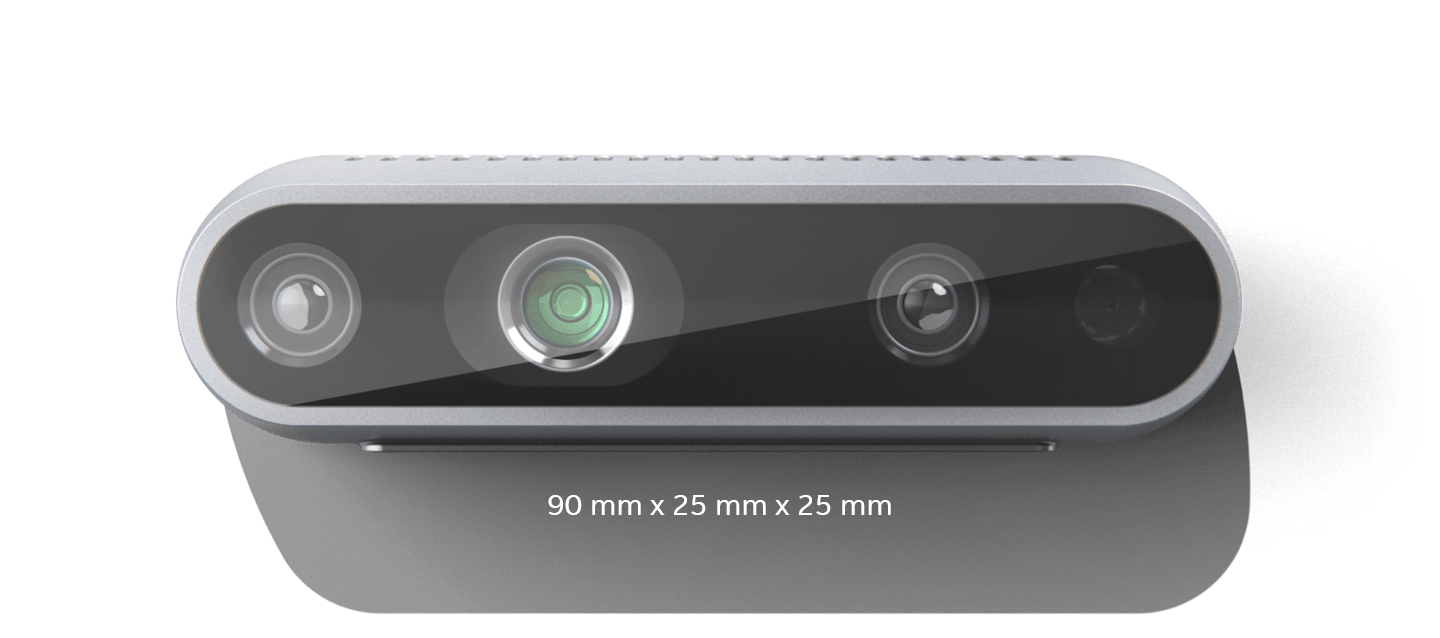
\includegraphics[width=0.6\linewidth]{435d}
\caption{Intel RealSense D435, Frontside}
\end{figure}

Die Kamera D435 von Intel hat ein breites Sichtfeld, einen globalen Shutter und einen Tiefensensor, der sich f\"ur Anwendungen mit schnellen Bewegungen eignet. Gerade durch ihr breites Sichtfeld eignet sich die Kamera fÃŒr Anwendungen in der Robotik, Virtual und Augmented Reality, bei Szenen wo es darum geht m\"oglichst viel zu sehen. Sie hat eine Reichweite bis zu 10 Meter. Das Intel RealSenseSDK bietet plattformunabh\"angig Unterst\"uzung bei der Umsetzung.
			
\begin{figure}[hbt!]
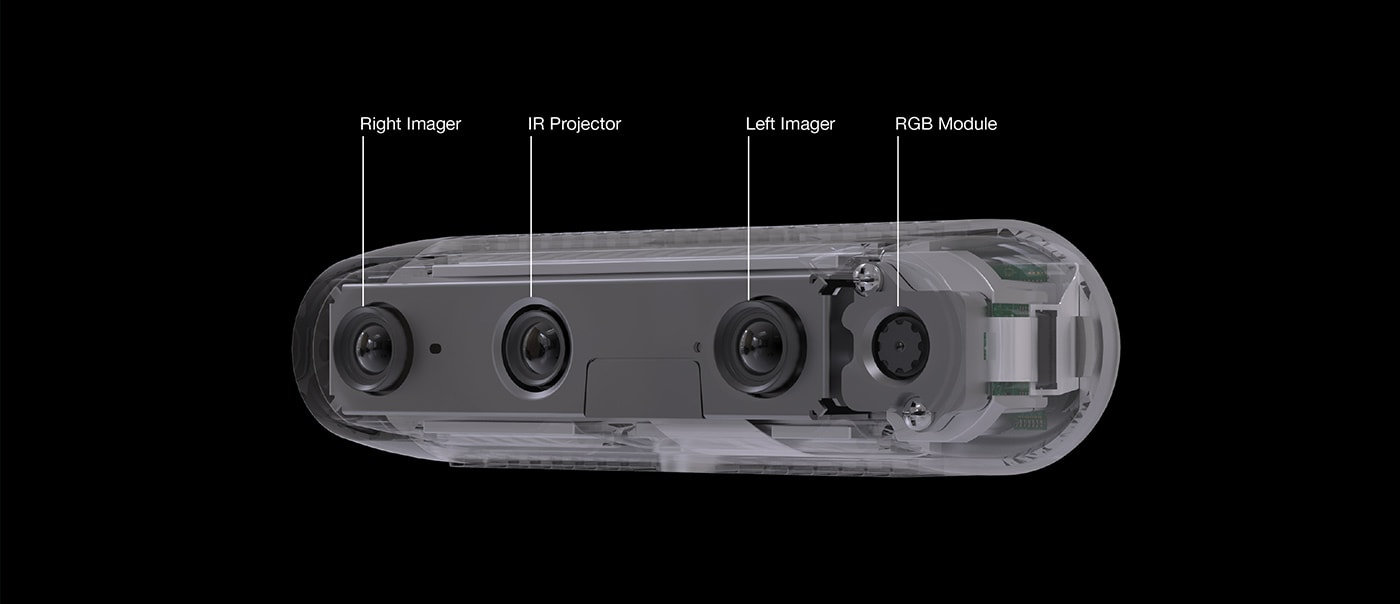
\includegraphics[width=0.6\linewidth]{435d_back}
\caption{Intel RealSense D435, Backside}
\end{figure}
			
Die Global-Shutter-Sensoren haben eine hohe Lichtempfindlichkeit bei schlechten Lichtverh\"altnissen und erm\"oglichen die Steuerung von Robotern auch in dunklen R\"aumen.
\cite{Intel}

\subsection{Software Komponenten}

\subsubsection{Intel RealSense Viewer}

Der Intel RealSense Viewer hat zwei Frames die er anzeigen kann, den RGB Frame und den Depth Frame. Die Abbildung zeigt einen Screenshot vom Depth Frame.

\begin{figure}[hbt!]
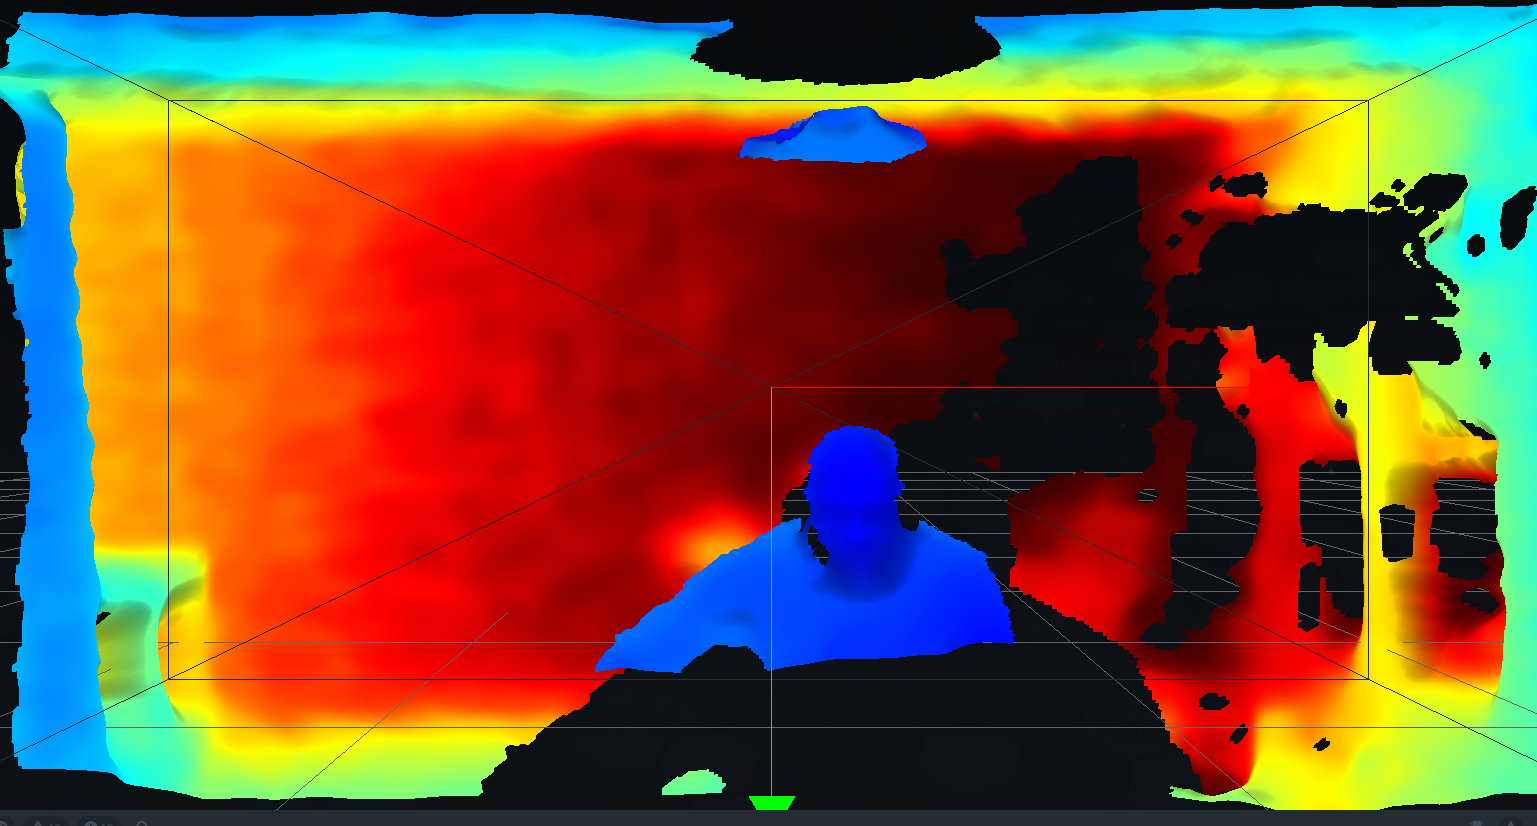
\includegraphics[width=0.6\linewidth]{depth_sensor}
\caption{Intel RealSense Viewer, Depth Frame}
\end{figure}
		
Die blauen Farbpixel zeigen einen nahen Bildpunkt, die roten Farbpixel einen entfernten Bildpunkt. F\"ur mein Projekt eignent sich dieser Viewer einzig dazu die verschiedenen Kameraeinstellungen auszuprobieren.
			
\subsubsection{Intel RealSenseSDK 2.0}

Intel hatte vor einigen Jahren eine f\"uhrende Rolle in Anwendungen im Bereich Augmented Reality. Mit dem Intel RealSenseSDK 2016, dem Vorgänger vom RealSenseSDK 2.0 gab es ein ToolKit welches Facetracking implementiert hatte. Die rechte und die linke Hand konnte beispielsweise seperat fürs Tracking angesteuert werden und sogar einzelne Finger einer Hand konnten getrackt werden. \\Ich habe noch versucht dieses "\"altere SDK zu installieren und dann mit einer \"alteren Unity Version zu verwenden. Leider ohne Erfolg. Intel hatte eine ganze Videoreihe dazu erstellt, welche aber heute vom Netz genommen wurden.\\
Intel schließt seine Abteilung rund um die RealSense-Kameras, die viele Jahre interessante, aber vom Markt kaum umgesetzte Lösungen hervorgebracht hatte. Sie passt nicht zum neuen Geschäftsmodell, welches rund um die Kernthemen von Intel aufgebaut und von dem neuen Foundry-Geschäft unterstützt wird.
\cite{ComputerBase}- \\ Das neue SDK 2.0 taugt dagegen nur noch wenig und eignet sich nicht f\"ur mein Projekt. Das Toolkit implementiert kein Facedetection für Unity Anwendungen.			

\subsubsection{Unity}

Unity ist eine Game Engine die von einer Open Source Community betreut und weiterentwickelt wird. Unity bietet f\"ur dieses Projekt ein anwendungsfreundliches Toll mit welchem die Transformationen der Objekte gemacht werden k\"onnen. \\ Dies w\"are auch mit OpenGL m\"oglich. OpenGL ist die eigentliche Mutter aller Grafik Softwares. \\In Unity ist es dann auch m\"oglich komplexe Objekte mit unterschiedlichen Oberfl\"achen und Texturen mit der gew\"unschten Lichtsituation darzustellen. 
\cite{Unity}
			
			
\subsubsection{Nuitrack}

Nuitrack stellt in ihrem SDK viele Anwendungen zur Verf\"ugung, diese sind aber auf 3 Minuten Spieldauer limitiert. Wahrscheinlich haben sie von Intel gelernt und haben ein Pricing welches f\"ur volle Anwendungen \$99.99 pro Jahr kostet. In der nächsten Abbildung sind alle implementierten Features dargestellt.

\begin{figure}[hbt!]
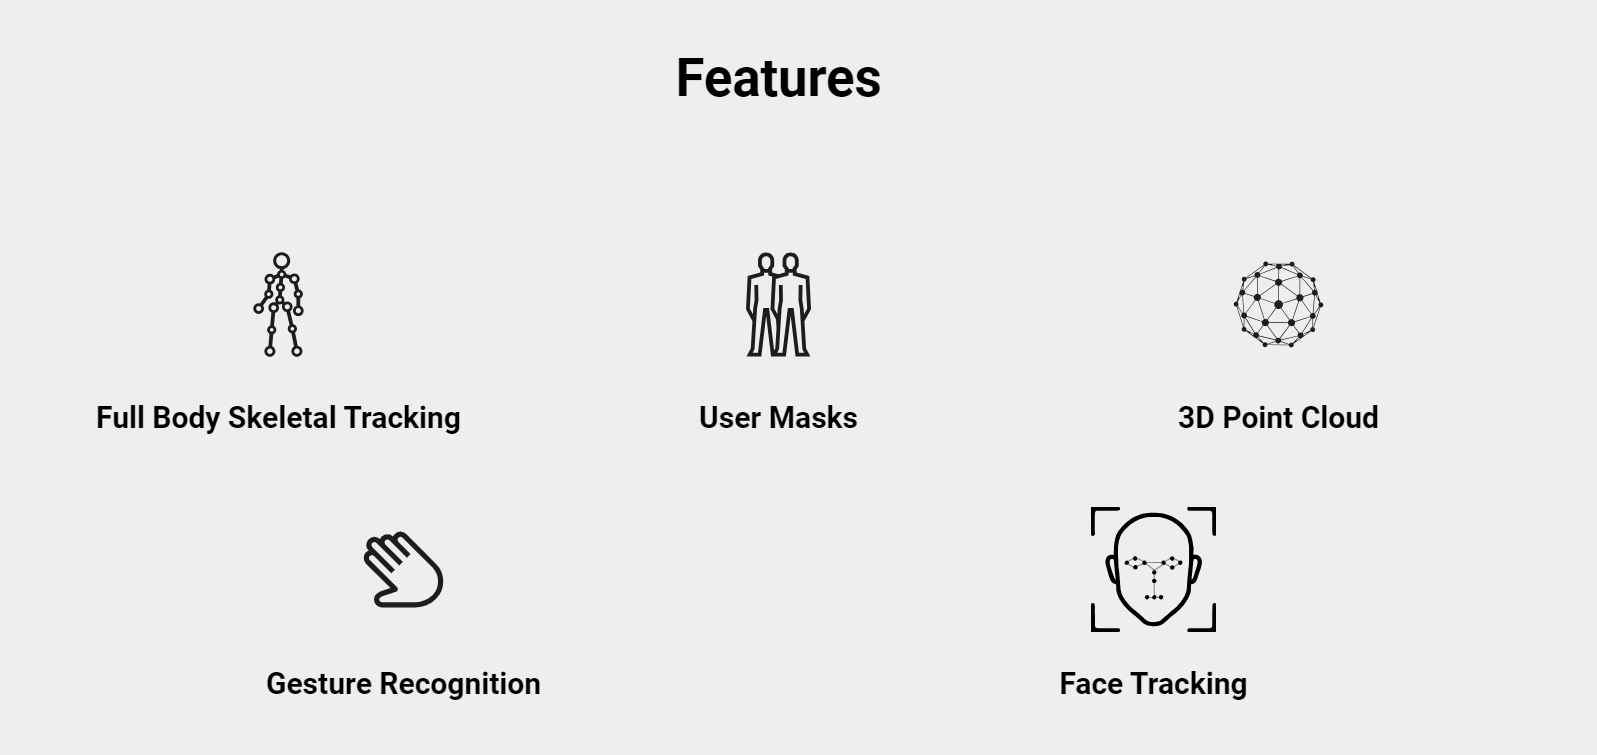
\includegraphics[width=0.6\linewidth]{nuitrack_features}
\caption{Nutitrack SDK, Features}
\end{figure}

Dieses SDK ist enorm m\"achtig und hat alles zu bieten, was ich für mein Projekt brauche. Wichtig für mein Projekt ist das Facetracking und das Full Body Skeletal Tracking. Die Nutirack SDK hat eine gute Anbindung zu Unity und ist gut domumentiert.
\cite{NuitrackSDK} 

\subsection{OpenCV}

OpenCV ist eine Open Source Computer Vision Grafik Library. In meinem Projekt benötige ich diese Library um ein bliebiges Polygon mit Seiten zu entzerren und als Rechteck darzustellen. Es gibt einen Wrapper für diese Library, welcher sich in Unity einbinden lässt. 
Dieser ist kostenpflichtig. Herr Hudritsch konnte mir eine Free Version geben, dies im Rahmen der Ausbildung.
Informationen zu OpenCV finden sich unter: https://opencv.org/ und für das Unity Plugin unter: https://enoxsoftware.com/opencvforunity/.
			
\subsection{Homographie}

\vspace{0.5in}

\begin{figure}[hbt!]
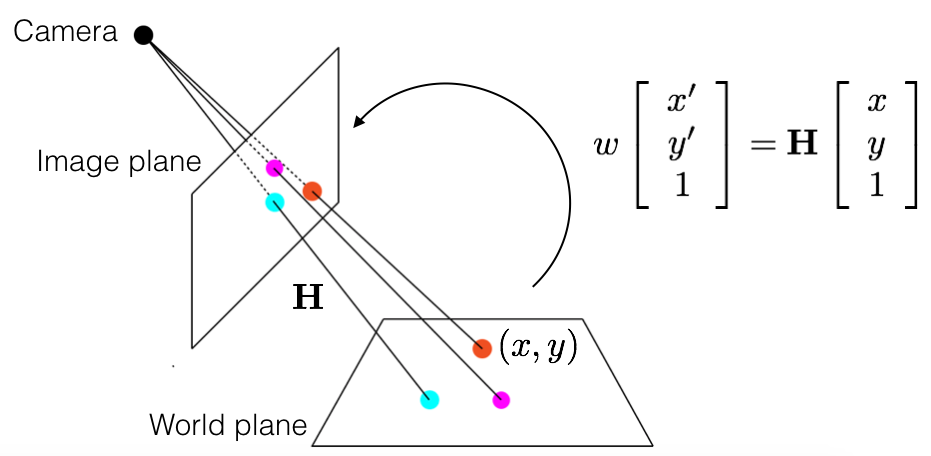
\includegraphics[width=0.6\linewidth]{homography}
\caption{Homographie, Visualisation}
\end{figure}
		
Die Homographie Matrix H beschreibt wie die Originalpunkte x,y zu liegen kommen in der Bildebene. Die Homographie Matrix ben\"otigt jeweils 4 Punkte in der Quellebene und die entsprechenden Punkte in der Zielebene. \\ 
		
			
\begin{figure}[hbt!]
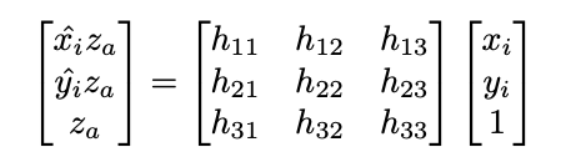
\includegraphics[width=0.6\linewidth]{homography_abbildung}
\caption{Homographie, Abbildungsgleichung}
\end{figure}
		
Diese 8 Punkte werden als Vektoren in einer Matrix A dargestellt. Die Matrixmultiplikation von A mit der Homographie Matrix die wir suchen, wird in einem Gleichungssystem von 8 Gleichungen und 8 Unbekannten gelöst.
			
			
\begin{figure}[hbt!]
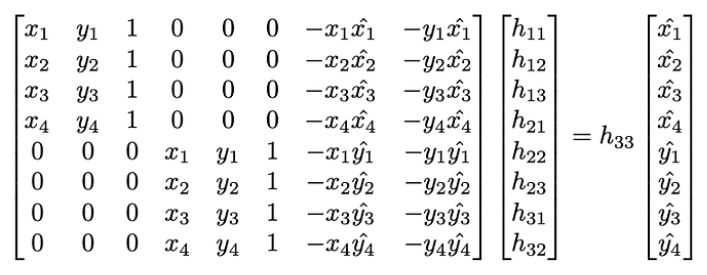
\includegraphics[width=0.6\linewidth]{homography_gleichungssystem}
\caption{Homographie, Gleichungssystem}
\end{figure}
		
Der Streckungsfaktor h33 zeigt, dass die Homographie Matrix noch skaliert werden kann. Im Default Fall wird h33 eins gesetzt.
\cite{OntarioTech}
\cite{HomographyEstimation}
			
\subsection{Kameramodell}

\vspace{0.5in}

Um auf die Eckpunkte vom Screen zu kommen, sollte es reichen, wenn wir die Position der Kamera, deren Rotationswinkel, sowie den Winkel vom Field of View und den Viewport der Kamera kennen. Weiter kennen wir die World Positions von den Eckpunkten vom Screen. Da der Screen statisch ist und sich nicht bewegt, können wir dieses Model ausser acht lassen. Was bleibt ist: der Viewport (1), die Projektion (2) (Kamera intrinsisch) und das Kamera-Modell (3) (Kamera extrinsisch oder View).
Unsere Abbildungsmatrix ist also:
Matrix m = (1) * (2) * (3)
Und mittels Anwendung auf die Eckpunkte vom Screen:
P1' = P1 * m
